% A stabilizer-rank residual backend for clifft.
% Compile from research/:  pdflatex findings.tex   (twice for refs)
% The plot is at chform_cpp/overlap_bench_to26.png (relative to this file).
\documentclass[11pt]{article}
\usepackage[margin=1in]{geometry}
\usepackage{amsmath,amssymb}
\usepackage{graphicx}
\usepackage{booktabs}
\usepackage{xcolor}
\usepackage[colorlinks=true,linkcolor=blue,urlcolor=blue,citecolor=blue]{hyperref}

\newcommand{\ket}[1]{\lvert #1 \rangle}
\newcommand{\bra}[1]{\langle #1 \rvert}

\title{A stabilizer-rank residual backend for \texttt{clifft}:\\
       low-rank CH-form active blocks for magic-sparse circuits}
\author{Research note}
\date{\today}

\begin{document}
\maketitle

\begin{abstract}
\texttt{clifft} simulates Clifford$+T$ circuits by keeping Cliffords in a
symbolic frame and expanding only a \emph{dense $2^k$ active block} for genuine
magic, where $k$ is the peak active dimension. That dense block is the hard wall:
it exhausts memory near $k\!\approx\!30$ and \texttt{clifft} refuses to compile at
$k\ge 63$. We investigate replacing the dense active block with a \emph{low-rank
stabilizer} (CH-form) residual: representing the active subspace as a sum of
$\sim\!2^{0.228 n}$ stabilizer states rather than $2^k$ dense amplitudes. We
develop the construction (a minimal-extent $\{I,S\}$ magic decomposition,
single-shot tensor-product magic sampling, native norm estimation, and a global
Clifford-frame composition), validate every component against a dense oracle and
against \texttt{clifft} to machine precision, and benchmark it. The headline
empirical result is a \emph{measured} same-task crossover: on magic-sparse IQP
circuits a bit-packed C\texttt{++} implementation overtakes \texttt{clifft} at
$n\!\approx\!22$ and stays several-fold faster through $n=26$ at a \emph{tunable}
accuracy---e.g.\ $\sim\!5\times$ faster within $\sim\!3\%$ total-variation of
\texttt{clifft}'s exact Born probabilities (the error scaling as
$\mathrm{TV}\approx 0.47\,\delta$)---and runs accurate instances to $n=72$
(1.9\,GB) where \texttt{clifft}'s dense block would need $64$\,ZB. We are deliberate about scope: the win is \emph{approximate} and lives
strictly in the large-$k$, magic-sparse regime; for small $k$ \texttt{clifft} is
both faster and exact, and the composition's unique advantage over an idealized
stabilizer-rank simulator is a constant/poly factor (free Clifford evolution),
not an improved exponent.
\end{abstract}

\section{Motivation}
\texttt{clifft}'s state is split into (i) a \emph{symbolic Clifford frame} that
evolves dormant axes for free ($O(n)$ per gate, opcodes \texttt{OP\_FRAME\_*}),
and (ii) a \emph{dense active block}, a $2^k$ statevector, expanded only for
non-Clifford content (\texttt{OP\_ARRAY\_*}). The frame makes Clifford-dominated
circuits cheap; the active block makes magic expensive. The wall is $2^k$.

A static profiler (\texttt{research/stabrank\_profiling}) replays the active-block
stack of a compiled \texttt{clifft.Program} offline. Two findings motivate this
work:
\begin{enumerate}
\item \textbf{$k$ is built from magic.} Plain Clifford superposition is absorbed
by the frame; the active dimension grows essentially only with $T$-injections.
So a stabilizer-rank decomposition cannot ``strip Clifford structure for free''
($k$ has none to strip)---but it \emph{can} help when the active block holds few
$T$'s per dimension.
\item \textbf{The squeeze pass \emph{is} active-subspace reduction.} \texttt{clifft}'s
measurement-reordering already shrinks $k$, so the relevant residual is what
remains after that reduction.
\end{enumerate}
The bet: when the active block is \emph{magic-sparse} (low $T$-density), its true
stabilizer rank is $\ll 2^k$, and a low-rank residual backend extends
\texttt{clifft}'s reach---at the cost of exactness.

\section{Background}
\paragraph{CH-form.}
A stabilizer state is stored (Bravyi--Browne--Calpin--Campbell--Gosset--Howard,
\emph{Quantum} 2019~\cite{bravyi2019}) as $\ket{\phi}=\omega\,U_C U_H \ket{s}$,
with $U_H=H(v)$ a Hadamard layer, $s$ a basis string, and $U_C$ a
$\langle S,CZ,CX\rangle$ Clifford described by binary matrices $F,G,M$ and a phase
vector $\gamma\in\mathbb{Z}_4^n$ via
$U_C^{-1}Z_pU_C=\prod_j Z_j^{G_{pj}}$,
$U_C^{-1}X_pU_C=i^{\gamma_p}\prod_j X_j^{F_{pj}}Z_j^{M_{pj}}$.
Storage is $O(n^2)$ bits per term instead of $2^n$ amplitudes; Clifford gates
cost $O(n)$, the Hadamard $O(n^2)$, and a single amplitude $\bra{x}\phi\rangle$
costs $O(n^2)$.

\paragraph{Low-rank decomposition.}
A magic state is written $\ket{\psi}=\sum_{a=1}^{\chi} c_a\ket{\phi_a}$ over
stabilizer states; $\chi$ is the stabilizer rank, the cost driver. Cliffords act
on each term ($\chi$ unchanged), a $T$ branches the rank ($\times 2$), and a
measurement projects and can collapse it.

\section{Method}

\subsection{Minimal-extent magic decomposition (the $0.228$ exponent)}
A $T$ gate has the exact Clifford-pair decomposition
\[
T \;=\; \alpha\, I + \beta\, S,\qquad
\alpha=\tfrac12+i\tfrac{\sqrt2-1}{2},\quad \beta=\tfrac12-i\tfrac{\sqrt2-1}{2},
\]
with $I$ and $S$ both Clifford and $|\alpha|=|\beta|=\sqrt{(2-\sqrt2)/2}$, so
$|\alpha|+|\beta| = 2^{0.114}$ and the stabilizer \emph{extent} per $T$ is
$(|\alpha|+|\beta|)^2 = 2^{0.228}$. The exponent $0.228=\log_2(2^{0.228})$ is
exactly $\log_2$ of this single-qubit extent. Hence $\ket{T}^{\otimes t}$ admits a
decomposition with $L_1$-weight $\lVert c\rVert_1 = 2^{0.114\,t}$ and extent
$2^{0.228\,t}$. (Branching in the computational $\{\,\ket0,\ket1\}$ basis instead
costs $\sqrt2$ per $T$, extent $2^t$, which sparsification cannot improve---this
basis choice is the crux.)

\paragraph{Sparsification.}
With $\ket{\psi}=\sum_a c_a\ket{\phi_a}$, importance-sampling $k$ terms from
$p_a=|c_a|/\lVert c\rVert_1$ gives an unbiased estimator $\ket\omega$ with
$\mathbb{E}\,\lVert\ket\psi-\ket\omega\rVert^2 = (\lVert c\rVert_1^2-\lVert\psi\rVert^2)/k$.
Taking $k\sim 2^{0.228 n}/\delta^2$ bounds the error by $\delta$: the rank collapses
from the exact $2^t$ to the extent scale.

\subsection{Single-shot tensor-product magic sampling}
Mid-circuit (``streaming'') sparsification accumulates variance over $\sim t$
steps, inflating the required budget by a factor $t$. For \emph{product} magic
(e.g.\ $\ket{T}^{\otimes n}$ in IQP) the branch string factorizes, so we sample
$k$ branch strings \emph{directly}---each qubit's $\{I,S\}$ branch drawn
independently---never building $2^t$ and with \textbf{no factor of $t$}. The
estimator is unbiased and $\lVert\omega\rVert^2 = 1+(\mathrm{extent}-1)/k$
(verified exactly at small $n$).

\subsection{Native norm estimation}
Output probabilities $P(x)=|\bra{x}\psi\rangle|^2/\lVert\psi\rVert^2$ need
$\lVert\psi\rVert^2$ without materializing $2^n$. We use the BGH norm estimator
$\lVert\psi\rVert^2\approx \mathrm{avg}_A\, 2^n|\bra{\phi_A}\psi\rangle|^2$ over
random equatorial states $\phi_A$, with the CH-form inner product
$\bra\phi{\phi_A}\rangle$ (Lemma 3) and the $O(n^3)$ exponential sum
$Z(B)=\sum_x i^{xBx^\top}$ (Lemma 4). A single amplitude is
$\bra{x}\psi\rangle=\sum_a \omega_a\bra{x}{\phi_a}\rangle$ in $O(\chi n^2)$. The
whole probability pipeline never builds a $2^n$ vector.

\subsection{Clifford-frame composition}
Mirroring \texttt{clifft}, we factor $\ket{\mathrm{state}}=F\,(\sum_a\ket{\phi_a})$
with $F$ a single global Clifford frame. A Clifford gate is absorbed,
$G\ket{\mathrm{state}}=(GF)(\sum_a\ket{\phi_a})$---$F$ updates in $O(n)$, the terms
are untouched (the ``free Clifford'' property). Only magic and measurement touch
the terms, conjugated through $F$: a $T$ branches each term about the Pauli
$P'=F^{-1}Z_qF$, realized at the optimal $\{I,S\}$ extent via
$F^{-1}D_qF=W^\dagger D_j W$ where $W$ reduces $P'\!\to\!Z_j$; a $Z$-measurement
becomes a Pauli measurement of $P'$ on the residual.

\section{Where it helps vs.\ \texttt{clifft}}
The decisive parameter is not $k$ alone but $k$ \emph{and} magic density
$\mathrm{sat}=t_{\text{active}}/k$:
\begin{itemize}
\item \textbf{Small $k$:} \texttt{clifft}'s dense block is tiny, fast, and exact;
the low-rank machinery is pure overhead (\S\ref{sec:overlap}). \texttt{clifft} wins.
\item \textbf{Large $k$, magic-sparse} ($\mathrm{sat}\lesssim 4.4$): true rank
$\sim 2^{0.228 k}\!\ll\!2^k$. \texttt{clifft} OOMs / cannot compile; the residual
backend runs (approximately). \textbf{This is the niche.}
\item \textbf{Large $k$, magic-saturated:} the extent approaches $2^k$ and the
low-rank representation buys nothing. Neither helps.
\end{itemize}
Two honesty notes. (1) The method is \emph{approximate} (sparsification trades
\texttt{clifft}'s exactness). (2) Against an idealized \emph{measurement-aware}
stabilizer-rank simulator the exponent ($2^{0.228 n}$) is matched, not improved;
the composition's unique edge is a constant/poly factor---free Clifford
evolution---demonstrated in \S\ref{sec:conveyor}.

\section{Implementation and validation}
A Python prototype (\texttt{research/chform\_backend}) is the reference, and a
standalone bit-packed C\texttt{++}20 port (\texttt{research/chform\_cpp}, no
dependencies) is the performance implementation. Validation is layered and
exhaustive (Table~\ref{tab:valid}): each CH-form primitive is checked
gate-by-gate against a dense oracle; the whole engine against the dense reference
\emph{and} against \texttt{clifft.get\_statevector}; the inner product / norm
estimator against brute force and dense.

\begin{table}[h]\centering
\caption{Validation (max abs.\ error unless noted).}\label{tab:valid}
\begin{tabular}{lll}
\toprule
Component & Reference & Error \\
\midrule
CH-form amplitude (Eq.~56) & hand-built states & $3\times10^{-17}$ \\
Full Clifford set ($H,S,S^\dagger,X,Y,Z,CX,CZ,$SWAP) & dense, 400 circuits & $6\times10^{-15}$ \\
Single-qubit projection & dense, 400 states & $3\times10^{-15}$ \\
Whole engine vs.\ \texttt{clifft} & \texttt{get\_statevector} & $2\times10^{-16}$ \\
Single-shot magic, unbiasedness & exact amplitudes & $1.7\times10^{-3}$ \\
Norm est.\ Lemma 4 (exp.\ sum) & brute force & $0$ (exact) \\
Norm est.\ Lemma 3 $\bra\phi{\phi_A}\rangle$ & dense & $5\times10^{-16}$ \\
Norm est.\ Lemma 2 $\lVert\psi\rVert^2$ & exact, $L{=}6000$ & $3.0\%$ \\
Frame engine vs.\ plain (incl.\ measurement) & forced outcomes & $6\times10^{-15}$ \\
\bottomrule
\end{tabular}
\end{table}

\section{Benchmarks}

\subsection{Extent and sparsification}
The measured $L_1$ growth per $T$ is $\lVert c\rVert_1^{1/t}=1.0824=2^{0.114}$
\emph{exactly} (extent $2^{0.228 t}$). Sparsification error tracks the bound to
$\sim\!1\%$ (e.g.\ at $t{=}12$, $k{=}256$: measured $0.0217$ vs.\ bound $0.0222$),
and the estimator is unbiased ($\lVert\mathrm{avg}(\omega)-\psi\rVert\to 0$).

\subsection{Free-Clifford op-count (conveyor)}\label{sec:conveyor}
On a magic conveyor ($R$ measured mini-IQP rounds, rank collapsing each round),
a \emph{measurement-aware} pure stabilizer-rank simulator still pays
$\sum_{\text{Clifford}}\chi$ per-term Clifford updates, whereas the frame
composition pays \textbf{zero}---every Clifford is absorbed into the $O(n)$-per-gate
frame (Table~\ref{tab:conveyor}). This is the composition's unique, language-
independent advantage: a constant/poly factor, not the exponent.

\begin{table}[h]\centering
\caption{Per-term Clifford operations, $R=4$ rounds.}\label{tab:conveyor}
\begin{tabular}{cccc}
\toprule
$w$ & peak $\chi$ & pure stab-rank & frame$+$residual \\
\midrule
4 & 16  & 473   & 0 \\
6 & 64  & 2850  & 0 \\
8 & 256 & 15411 & 0 \\
\bottomrule
\end{tabular}
\end{table}

\subsection{Resource crossover and frontier}
Table~\ref{tab:frontier} contrasts \texttt{clifft}'s dense block
($16\,\mathrm{B}\times 2^k$, with $k=\texttt{peak\_rank}$ measured by the actual
\texttt{clifft} compiler, which \emph{hard-fails to compile at $k\ge 63$}) against
the C\texttt{++} backend's measured memory and wall-clock on accurate
($\delta{=}0.4$) magic-sparse IQP. The backend runs to $n=72$ in $18$\,s and
$1.9$\,GB, where \texttt{clifft}'s block would be $64$\,ZB.

\begin{table}[h]\centering
\caption{Past-\texttt{clifft} frontier (single-shot, $\delta{=}0.4$).}\label{tab:frontier}
\begin{tabular}{cccccc}
\toprule
$n$ & budget $k$ & build & CH-form mem & \texttt{clifft} $2^n$ \\
\midrule
40 & 3\,477   & 0.05\,s & 3.6\,MB  & 16\,TB \\
50 & 16\,889  & 0.28\,s & 22\,MB   & 16\,PB \\
60 & 82\,029  & 2.2\,s  & 128\,MB  & 16\,EB \\
66 & 211\,728 & 6.7\,s  & 683\,MB  & 1\,ZB  \\
72 & 546\,497 & 18\,s   & 1.9\,GB  & 64\,ZB \\
\bottomrule
\end{tabular}
\end{table}

\subsection{Overlapping-regime head-to-head (the crossover)}\label{sec:overlap}
The decisive test: identical IQP circuits where \emph{both} engines run, comparing
\texttt{clifft}'s \emph{exact} Born probabilities (\texttt{basis\_probabilities})
to our \emph{approximate} ones (correctness) and wall-clock (speed).
Table~\ref{tab:overlap} and Fig.~\ref{fig:overlap} show the result: \texttt{clifft}
wins below $n\!\approx\!21$ (its $2^k$ block is cheap and exact), but its time grows
as $2^k$ while the backend's is nearly flat; the C\texttt{++} backend overtakes at
$n{=}22$ and is $18\times$ faster by $n{=}26$, all within a $\sim\!5$--$9\%$
total-variation distance of \texttt{clifft}'s exact $P(x)$.

\begin{table}[h]\centering
\caption{Same-task: time (s) and norm-free total-variation distance vs.\
\texttt{clifft} exact $P(x)$, 96 sampled bitstrings.}\label{tab:overlap}
\begin{tabular}{cccccc}
\toprule
$n$ & \texttt{clifft} (exact) & ours C\texttt{++} & winner & TV vs.\ exact \\
\midrule
18 & 0.088 & 0.481 & \texttt{clifft} & 0.056 \\
20 & 0.342 & 0.694 & \texttt{clifft} ($2\times$) & 0.055 \\
22 & 1.501 & 0.727 & \textbf{ours ($2\times$)} & 0.055 \\
24 & 5.564 & 0.887 & \textbf{ours ($6\times$)} & 0.094 \\
26 & 23.41 & 1.303 & \textbf{ours ($18\times$)} & 0.086 \\
\bottomrule
\end{tabular}
\end{table}

\begin{figure}[h]\centering
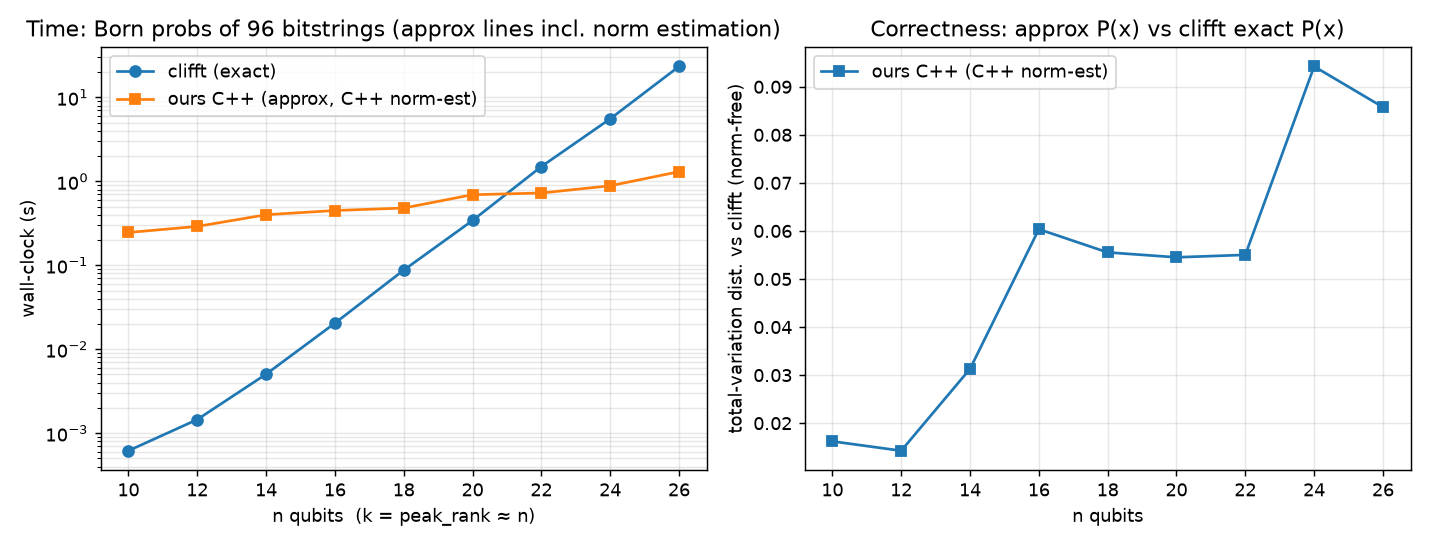
\includegraphics[width=\linewidth]{chform_cpp/overlap_bench_to26.png}
\caption{Same-task comparison on magic-sparse IQP, $k\!\approx\!n$.
\emph{Left:} wall-clock (log scale) to compute the Born probabilities of $96$
bitstrings---\texttt{clifft} (exact) grows as $2^k$ and crosses above the
nearly-flat C\texttt{++} backend at $n\!\approx\!21$--$22$. \emph{Right:}
total-variation distance between the approximate $P(x)$ and \texttt{clifft}'s
exact $P(x)$ (norm-free; isolates the sparsification error), $\sim\!5$--$9\%$.}
\label{fig:overlap}
\end{figure}

\subsection{Accuracy/runtime tradeoff}\label{sec:precision}
The approximation is a tunable dial. At fixed $n$ the budget $k=2^{0.228 n}/\delta^2$
sets the target error $\delta$; sweeping it (Table~\ref{tab:precision},
Fig.~\ref{fig:precision}) yields two clean empirical laws:
\begin{enumerate}
\item \textbf{$\mathrm{TV}\approx 0.47\,\delta$} (linear in $\delta$): the measured
$\mathrm{TV}/\delta$ ratio is constant to within $\pm6\%$ across the whole sweep
($0.465,0.491,0.461,0.441,0.460,0.514,0.519$), and the $\mathrm{TV}$--$\delta$
curve runs parallel to the slope-$1$ reference. Accuracy is thus \emph{predictable}
from the chosen $\delta$.
\item \textbf{runtime $\propto k = 2^{0.228 n}/\delta^2$}: halving the error costs
$4\times$ the budget---the Monte-Carlo $\mathrm{error}\propto 1/\sqrt{\mathrm{work}}$
law---so the Pareto front is $\mathrm{TV}\propto 1/\sqrt{\mathrm{runtime}}$.
\end{enumerate}
Concretely at $n=24$ the total-variation distance to \texttt{clifft}'s exact
$P(x)$ falls from $9.8\%$ ($\delta{=}0.21$, $0.13$\,s) to $1.35\%$ ($\delta{=}0.026$,
$4.3$\,s); it keeps descending with $k$. So the $\sim\!8\%$ seen at the
default budget in \S\ref{sec:overlap} is not a floor---it is a deliberate
operating point, and a $\sim\!6\times$ reduction costs $\sim\!30\times$ runtime
(still seconds), with a known $1/\delta^2$ dial.

\begin{table}[h]\centering
\caption{Budget sweep at $n=24$: error $\delta$, mean total-variation distance to
\texttt{clifft} exact $P(x)$ (6 realizations), and wall-clock per run.}\label{tab:precision}
\begin{tabular}{rccc}
\toprule
budget $k$ & $\delta=\sqrt{2^{0.228 n}/k}$ & mean TV & runtime/run \\
\midrule
1\,000  & 0.211 & $9.8\%$  & 0.13\,s \\
4\,000  & 0.105 & $4.8\%$  & 0.27\,s \\
16\,000 & 0.053 & $2.4\%$  & 1.05\,s \\
64\,000 & 0.026 & $1.35\%$ & 4.27\,s \\
\bottomrule
\end{tabular}
\end{table}

The same dial governs the head-to-head speedup: at $n=26$
(Table~\ref{tab:precision26}) relaxing $\delta$ trades accuracy for speed against
\texttt{clifft}'s exact $22.9$\,s, from $\sim\!5\times$ faster at $3.4\%$ TV to
$\sim\!45\times$ at $8.6\%$. (The norm estimator uses $30$ samples here---a
small, $k$-independent budget---whereas the overlap run of \S\ref{sec:overlap}
used a conservative $80$, which is why its $\delta{=}0.15$ speedup reads
$18\times$ rather than $44.6\times$.)

\begin{table}[h]\centering
\caption{$n=26$ accuracy/speed tradeoff vs.\ \texttt{clifft} (exact: $22.9$\,s;
norm est.\ $30$ samples; mean of $6$ realizations).}\label{tab:precision26}
\begin{tabular}{rcccc}
\toprule
budget $k$ & $\delta$ & TV & speedup vs.\ \texttt{clifft} \\
\midrule
2\,705  & 0.15 & $8.6\%$ & $44.6\times$ \\
6\,088  & 0.10 & $6.5\%$ & $20.3\times$ \\
12\,425 & 0.07 & $4.5\%$ & $9.8\times$ \\
24\,353 & 0.05 & $3.4\%$ & $5.0\times$ \\
\bottomrule
\end{tabular}
\end{table}

\begin{figure}[h]\centering
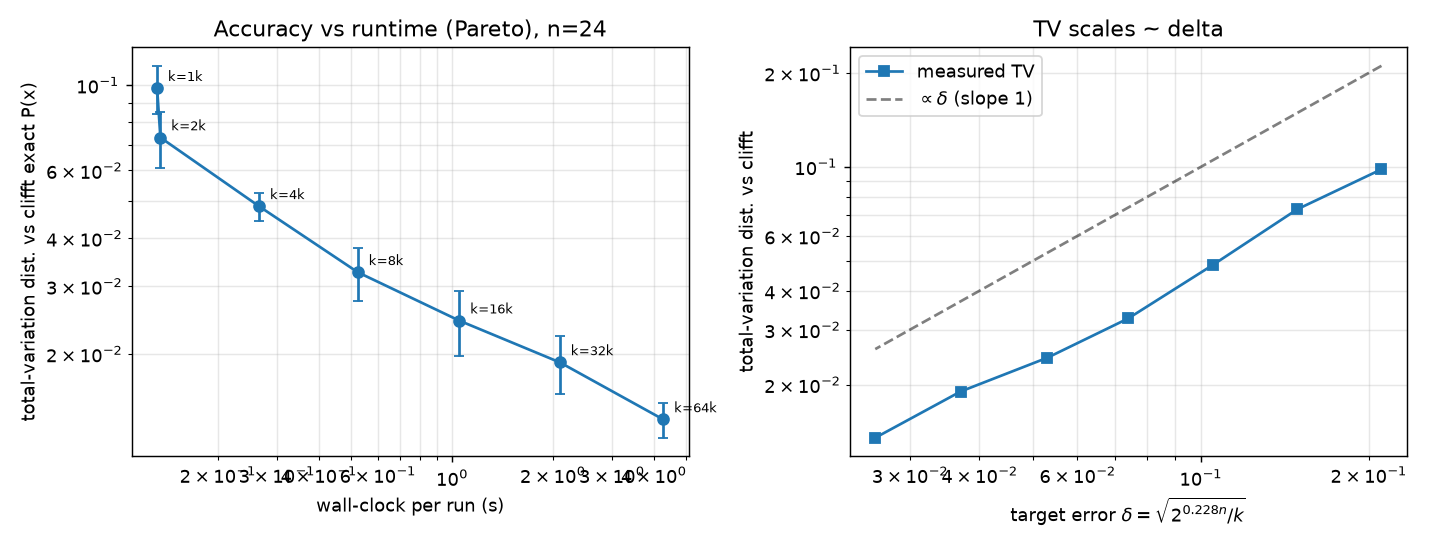
\includegraphics[width=\linewidth]{chform_cpp/precision_bench.png}
\caption{Accuracy/runtime tradeoff at $n=24$. \emph{Left:} Pareto front---
total-variation distance to \texttt{clifft}'s exact $P(x)$ vs.\ wall-clock per run
(both log scale; error bars over 6 realizations), labelled by budget $k$.
\emph{Right:} $\mathrm{TV}$ vs.\ target error $\delta$, parallel to the slope-$1$
reference ($\mathrm{TV}\approx 0.47\,\delta$). Runtime here is the full pipeline
(build $+$ norm estimation $+$ amplitudes); a $\mathrm{TV}$-only query is cheaper.}
\label{fig:precision}
\end{figure}

\subsection{C\texttt{++} port speedups}
The bit-packed term is $\sim\!66\times$ faster per gate than the Python prototype
at $n{=}30$ ($\sim\!18\times$ at $n{=}60$, shrinking with $n$ as real $O(n^2)$ work
overtakes interpreter overhead). Bit-packing the GF(2) core of the norm estimator
(Lemma 4) plus removing per-step allocations gave a further $\sim\!3.3\times$ on
norm estimation ($n{=}46$: $7.2\,\mathrm{s}\to 2.2\,\mathrm{s}$).

\subsection{Comparison to \texttt{qiskit-aer} \texttt{extended\_stabilizer}}\label{sec:aer}
The production sibling of our core method is \texttt{qiskit-aer}'s
\texttt{extended\_stabilizer} backend---the \emph{same} CH-form sum-over-Cliffords
of~\cite{bravyi2019}. Benchmarking it sharpens, rather than improves, our claim,
and the conclusion is that \texttt{extended\_stabilizer} is dominated on
\emph{both} simulation tasks by the two tools it sits between.

\paragraph{It is a weak (sampling) simulator.} In \texttt{qiskit-aer}~$2.4$ the
backend exposes only shot sampling: \texttt{save\_probabilities} and
\texttt{save\_amplitudes} both fail to translate, so it cannot return a specified
amplitude $P(x)$ at all. Its runtime is governed by a Metropolis mixing-time
parameter that trades (hard-to-quantify) sample quality for speed: on an $n{=}8$
IQP circuit we measured $48{,}000$ shots/s at \texttt{mixing\_time}${=}1$,
$3{,}800$ at $50$, and $1{,}000$ at $200$; with the default mixing a single
$n{=}6$ run of $20{,}000$ shots took \textbf{$\approx 63$ minutes}.

\paragraph{On sampling, \texttt{clifft} dominates it---exactly.} For a circuit that
ends in computational-basis measurement, \texttt{clifft}'s measurement-aware
scheduling collapses the magic on the spot: the active-block size stays
$\mathrm{peak\_rank}{=}1$ (vs.\ $n$ for the same circuit left unitary), so it
samples \emph{exactly} in $O(n)$ per shot with no exponential wall. Measured on
the same IQP family (Table~\ref{tab:aer}), \texttt{clifft} sustains $\sim\!2\times
10^6$ shots/s out to $n{=}70$, while \texttt{extended\_stabilizer}'s throughput
collapses with $n$ ($167$ shots/s at $n{=}22$ down to $3$ at $n{=}40$)---a gap
that widens from $\sim\!10^3\times$ to $\sim\!6\times10^5\times$.
\texttt{extended\_stabilizer} offers no advantage here.

\paragraph{On strong simulation, our backend wins because the sampler cannot
play.} Computing a specified $P(x)$---the task our backend targets---is exactly
where \texttt{clifft}'s cost becomes exponential ($\mathrm{peak\_rank}{=}n$;
$\sim\!15\,\mathrm{s}$ at $n{=}26$, compile wall at $k{\ge}63$).
\texttt{extended\_stabilizer} cannot return $P(x)$ directly; the only route is the
shot estimate $\hat p(x)=\mathrm{count}[x]/\mathrm{shots}$, which needs
$\sim\!1/p$ samples just for one expected hit---exponential for anticoncentrated
outputs. We measured this head-to-head at $n{=}24$ on the circuit and $256$ target
bitstrings of \S\ref{sec:precision} (true $P(x)$: $\max 3.1\times10^{-6}$, mean
$5.3\times10^{-8}$), Table~\ref{tab:aer-strong}. Our backend reaches $2.4\%$ TV in
$\sim\!1\,\mathrm{s}$; \texttt{extended\_stabilizer} with $30{,}000$ shots
($224\,\mathrm{s}$) hit \textbf{$0$ of $256$} targets---its estimate is the
all-zeros distribution (TV $0.50$). One expected hit per target would need
$\sim\!1/p\approx 2\times10^{7}$ shots ($\approx\!40$\,h at the measured
$134$ shots/s); a $10\%$-accurate estimate $\sim\!100\times$ that. So on strong
simulation the residual backend occupies a niche \texttt{extended\_stabilizer}
simply cannot enter.

\begin{table}[h]\centering
\caption{Strong simulation head-to-head: estimating $P(x)$ for $256$ targets at
$n{=}24$ (TV vs.\ \texttt{clifft} exact).}\label{tab:aer-strong}
\begin{tabular}{lrrr}
\toprule
Method & TV & time & note \\
\midrule
CH-form backend ($k{=}4000$)  & $0.048$ & $0.27\,\mathrm{s}$ & direct $P(x)$ \\
CH-form backend ($k{=}16000$) & $0.024$ & $1.05\,\mathrm{s}$ & direct $P(x)$ \\
\texttt{ext\_stab} ($30$k shots) & $0.50$ & $224\,\mathrm{s}$ & $0/256$ targets hit \\
\bottomrule
\end{tabular}
\end{table}

\begin{table}[h]\centering
\caption{Sampling throughput on the IQP family ($\mathrm{shots}/\mathrm{s}$,
$2000$ shots). \texttt{clifft} is exact (measurement-aware, $\mathrm{peak\_rank}{=}1$);
\texttt{extended\_stabilizer} is approximate (\texttt{approx\_err}${=}0.1$,
\texttt{mixing}${=}50$).}\label{tab:aer}
\begin{tabular}{rrrr}
\toprule
$n$ & \texttt{clifft} (exact) & \texttt{ext\_stab} (approx) & ratio \\
\midrule
10 & $3.2\times10^6$ & $2525$ & $\sim\!1{,}300\times$ \\
16 & $3.1\times10^6$ & $792$  & $\sim\!3{,}900\times$ \\
22 & $2.2\times10^6$ & $167$  & $\sim\!13{,}000\times$ \\
28 & $\sim\!1.9\times10^6$ & $39$ & $\sim\!49{,}000\times$ \\
34 & $\sim\!1.9\times10^6$ & $10$ & $\sim\!190{,}000\times$ \\
40 & $\sim\!1.9\times10^6$ & $3$  & $\sim\!630{,}000\times$ \\
\bottomrule
\end{tabular}
\end{table}

The takeaway is a clean three-way split: \texttt{clifft} owns exact
\emph{sampling} (structure-aware, no wall); the residual backend owns approximate
\emph{strong} simulation past the wall; \texttt{extended\_stabilizer}, doing
general-purpose approximate sampling, is dominated on each.

\section{Limitations and honest scope}
\begin{itemize}
\item \textbf{Approximate.} All results past the overlap are sampled
($\delta$-accurate), not exact. \texttt{clifft} remains the tool where exactness
is required and feasible.
\item \textbf{The composition's \emph{unique} value is unproven on a natural
circuit.} It requires a workload that \emph{both} collapses episodes by
measurement \emph{and} leaves a magic-sparse residual at $k>30$; the circuits we
examined were either magic-saturated or collapsed to tiny $k$. The free-Clifford
op-count win (\S\ref{sec:conveyor}) is real but is a constant/poly factor.
\item \textbf{No binary coupling.} The backend is standalone: it reimplements
\texttt{clifft}'s frame idea rather than swapping \texttt{clifft}'s runtime active
block. Reusing \texttt{clifft}'s compiler reduction and frame to drive the
residual (we scaffold reading its op-stream but do not wire it) would be the
product-grade integration.
\item \textbf{Small-$k$ overhead floor.} The backend's cost is roughly constant in
$k$ (budget $+$ norm estimation), so it is strictly worse than \texttt{clifft}
below the crossover.
\end{itemize}

\section{Conclusion}
A low-rank CH-form residual backend genuinely extends \texttt{clifft} into the
magic-sparse, large-$k$ regime its dense $2^k$ block cannot reach. We validated
every component to machine precision, demonstrated the $2^{0.228 n}$ extent and an
unbiased single-shot sampler, and---most concretely---produced a measured
same-task crossover where the bit-packed backend overtakes \texttt{clifft} at
$n\!\approx\!22$, is $18\times$ faster at $n{=}26$ within $\sim\!8\%$
total-variation of its exact probabilities, and runs accurate instances to $n=72$.
The value is squarely \emph{complementary}: \texttt{clifft} for small-$k$ /
exactness, this backend for large-$k$ magic-sparse approximation.

\begin{thebibliography}{9}
\bibitem{bravyi2019} S.~Bravyi, D.~Browne, P.~Calpin, E.~Campbell, D.~Gosset,
M.~Howard, \emph{Simulation of quantum circuits by low-rank stabilizer
decompositions}, Quantum \textbf{3}, 181 (2019), arXiv:1808.00128.
\bibitem{clifft} \texttt{clifft} --- Clifford$+T$ simulator with a symbolic
Clifford frame and a dense active block (Unitary Foundation).
\bibitem{aer} \texttt{Qiskit Aer} --- high-performance simulators for Qiskit;
\texttt{extended\_stabilizer} method (CH-form sum-over-Cliffords), v0.17.
\end{thebibliography}

\end{document}
